\chapter{Developer Documentation} % Developer guide
\label{ch:impl}

Histopathologic Cancer Detection program is divided into four major segments (\textcolor{red}{\autoref{fig:dirdiag}}):
\begin{enumerate}
	\itemsep 0em
	\item Data - includes dataset creation, analysis and visualization
	\item Networks - includes creation, training, testing of convolutional neural networks
	\item Experiments - includes hyperparameter tuning, network performance assessment and visualization
	\item Graphical User Interface - includes creation of all application windows and their interconnection
\end{enumerate}

\begin{figure}[h]
	\centering
	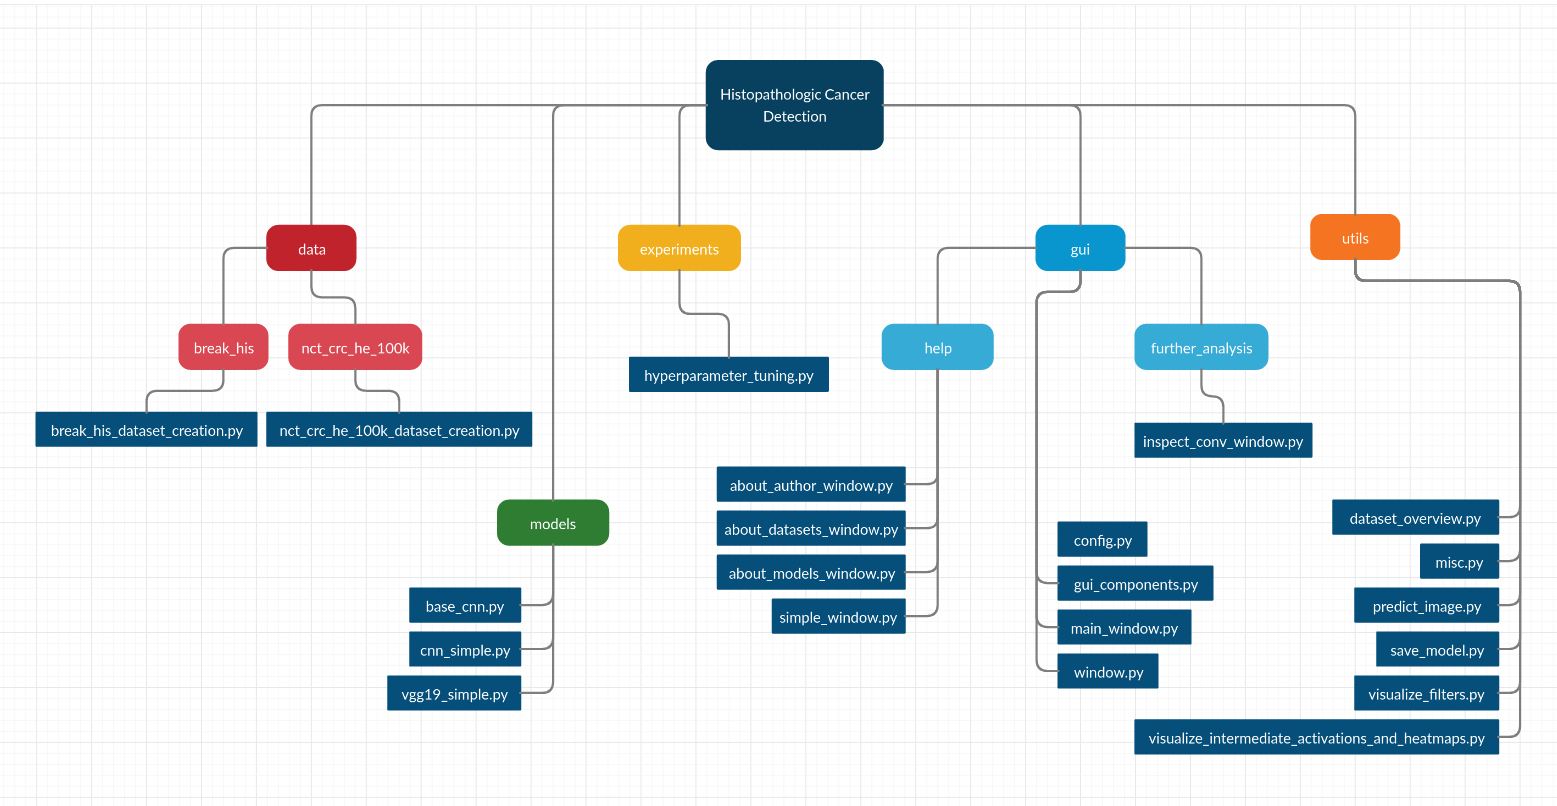
\includegraphics[scale=1.15]{directory_diagram.jpg}
	\caption{Diagram of directories and scripts of Histopathologic Cancer Detection}
	\label{fig:dirdiag}
\end{figure}

\section{Use-Case Diagram}

One of the main goals of the Histopahtologic Cancer Detection program was the ease of use, i.e. straightforward graphical user interface which makes complex operations look quite simple and effortless. Even though there are extremely advanced algorithms with millions of parameters behind the program, GUI was made in such a way that everyone can use it. 

First step is loading the image and selecting tissue type (breast or colorectal tissue), after which classification is being done. At every step of the way, current work can be saved, and new image can be loaded to start the process from scratch. After the classification, it is possible to visualize network representations and perform further analysis of the results by visualizing layer activations, network filters and heatmap (\textcolor{red}{\autoref{fig:usecase}}).

\begin{figure}[h]
	\centering
	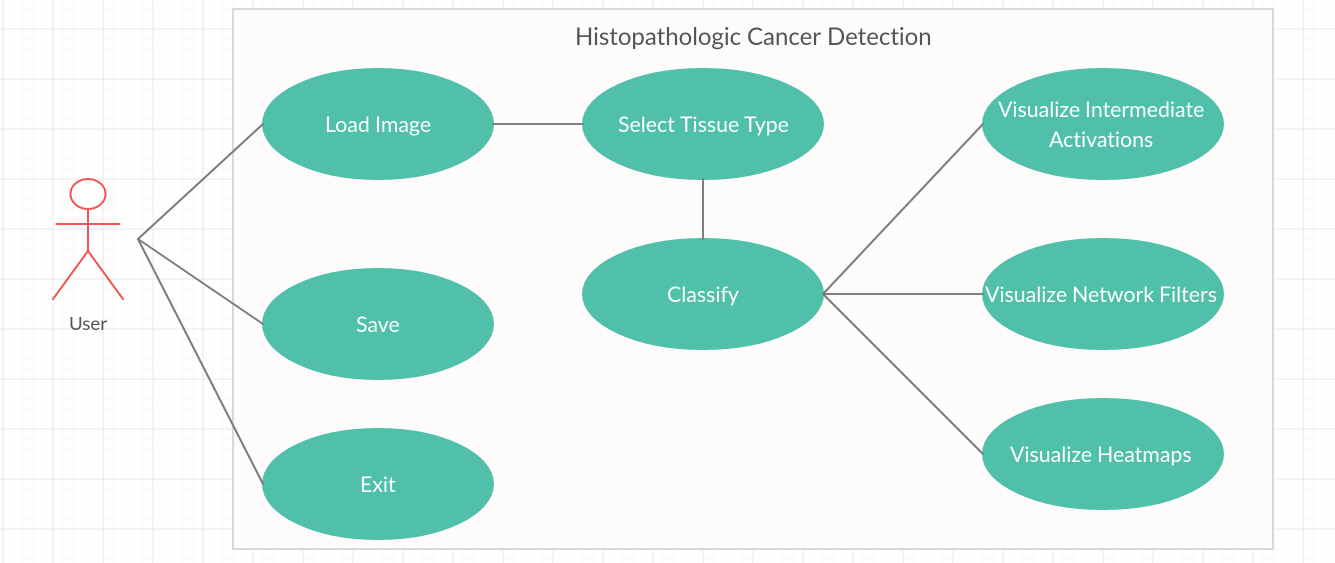
\includegraphics[scale=1]{use_case.jpg}
	\caption{Use-Case Diagram of Histopathologic Cancer Detection}
	\label{fig:usecase}
\end{figure}

\section{Class Diagrams}

Classes of Histopathologic Cancer Detection can be divided into two main components: neural network classes and window classes.

Window class is the base class of all window classes, and it implements common methods, such as setting up window size and central widget. On the other side, Main Window class is the central point of GUI, as it is window which opens when program is run, and every other window is invoked from it (\textcolor{red}{\autoref{fig:class2}}). Window classes, along with their attributed and methods, will be discussed in detail in Section \textcolor{red}{\ref{gui}}.

\begin{figure}[h]
	\centering
	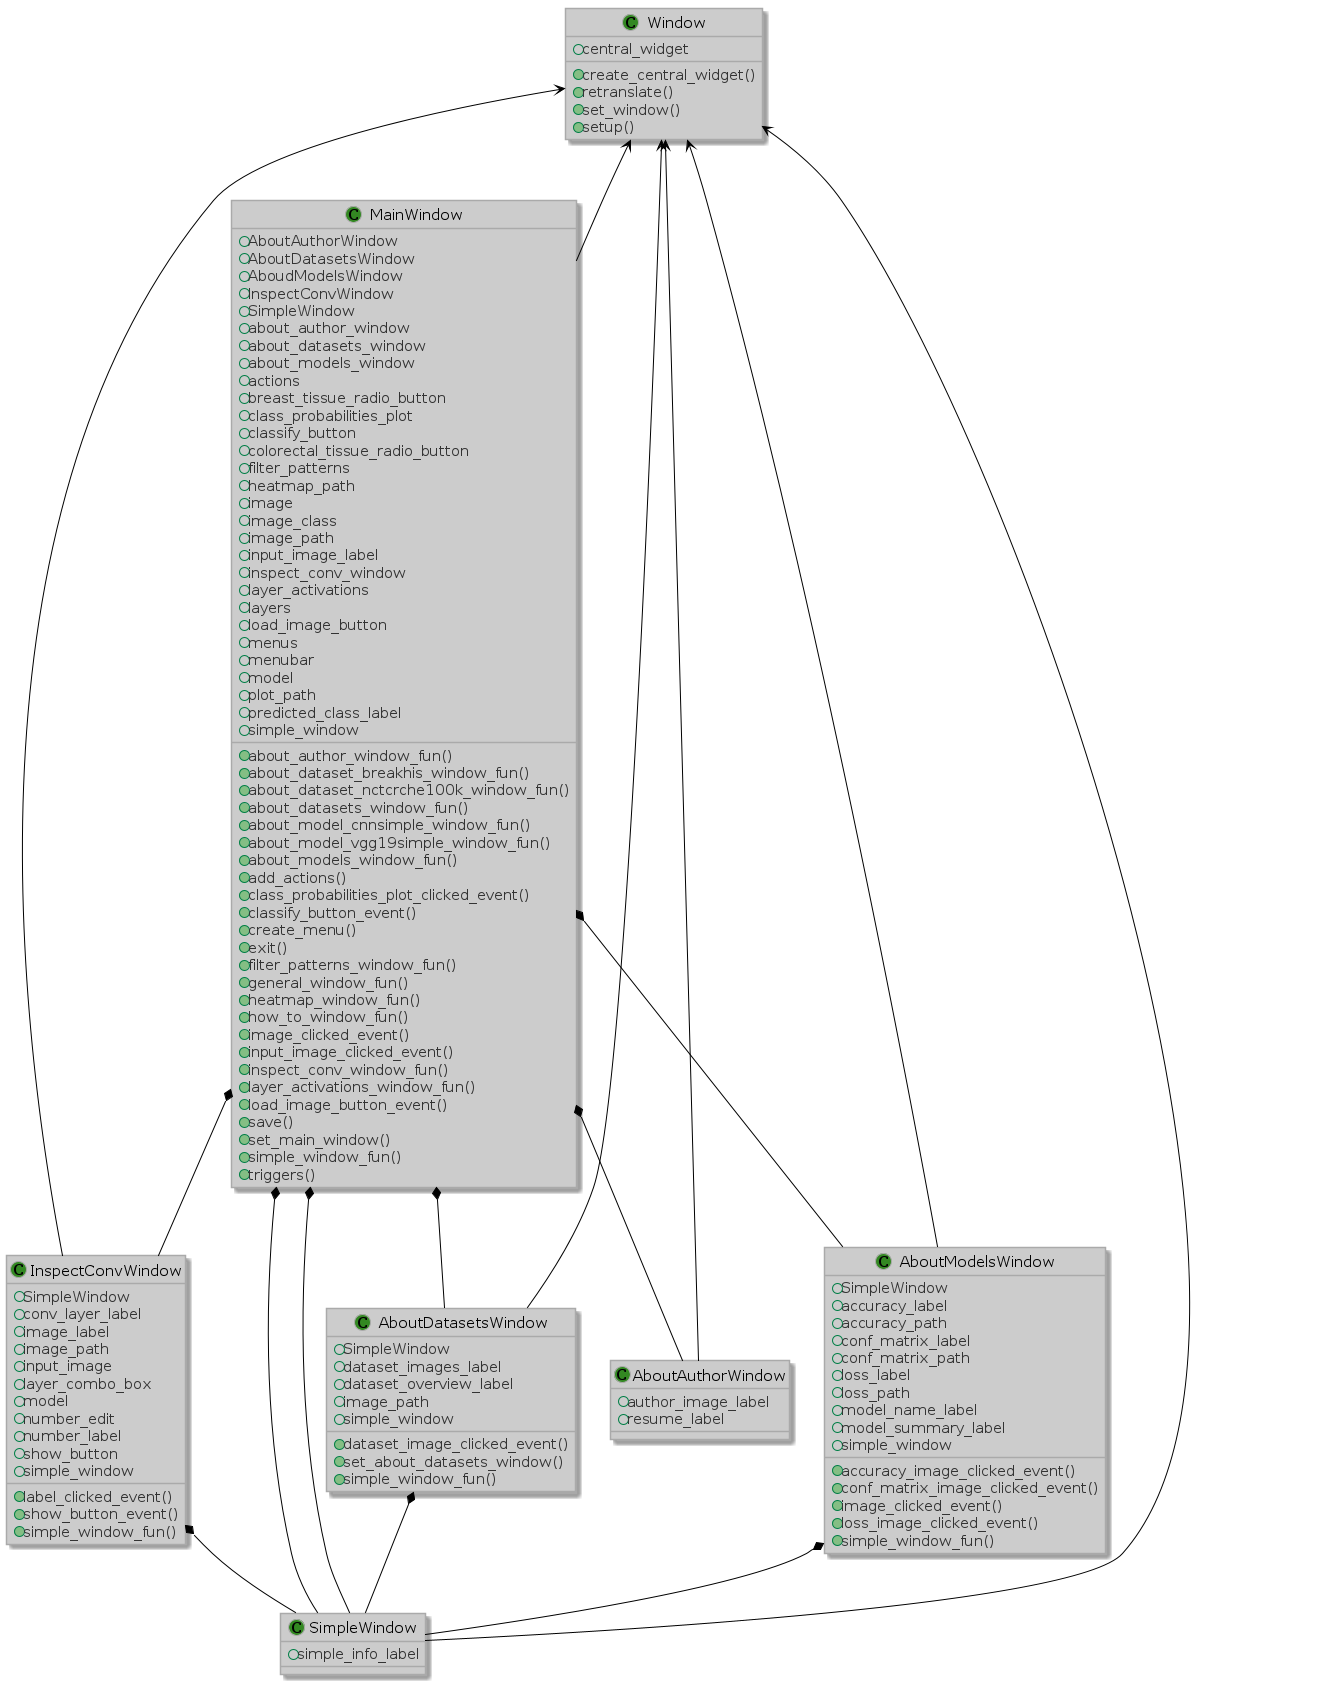
\includegraphics[scale=0.3]{main_class_diagram.png}
	\caption{Class Diagram of Window classes of Histopathologic Cancer Detection}
	\label{fig:class2}
\end{figure}

\clearpage

BaseCNN class is the common class of all neural network classes, and it contains common attributes, such as dataset name, network name, compile parameters, and common methods, such as creation of data generators, compilation and training of the network. Neural network classes will be discussed in more detail in Section \textcolor{red}{\ref{cnn}}

\begin{figure}[h]
	\centering
	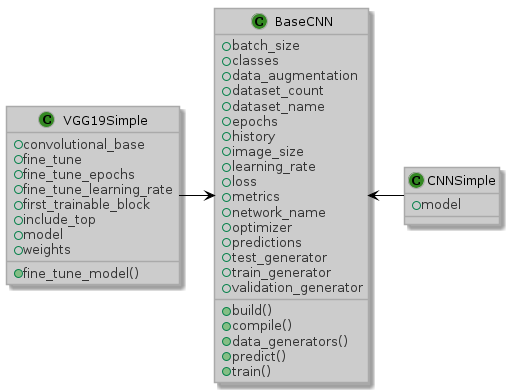
\includegraphics[scale=0.4]{nets_class_diagram.png}
	\caption{Class Diagram of Neural Network classes of Histopathologic Cancer Detection}
	\label{fig:class1}
\end{figure}

\section{Creation of Datasets}

Performance and accuracy of convolutional neural networks relies largely on datasets, i.e. on quality of available data, dataset size, class balance, etc. But before feeding data to the network, when using Keras API, certain dataset structure must be satisfied. More precisely, dataset must have following structure: train, validation and test directories, each with identical subdirectories for each class. Scripts responsible for creation of required directory structure are:
\begin{itemize}
	\itemsep 0em
	\item \emph{\textbf{break\_his\_dataset\_creation.py}},
	\item \emph{\textbf{nct\_crc\_he\_100k\_dataset\_creation.py}}.
\end{itemize} 
They work by extracting datasets downloaded from \cite{breakhis_bib}, \cite{nctcrche100k_bib}, creating necessary directory tree and distributing images between created subdirectories. After executing scripts, datasets are ready to be fed into convolutional neural networks in order to train them, but before that, neural network architecture is to be built.
\clearpage

\section{Convolutional Neural Networks} \label{cnn}

Convolutional Neural Networks for image classification take image as an input, \textbf{process} it, and output category to which that image belongs. Processing part consists of a series of layers through which we propagate image in order to learn features, which in turn determine to which class an image belongs. (\textcolor{red}{\autoref{fig:cnn1}}).

\begin{figure}[h]
	\centering
	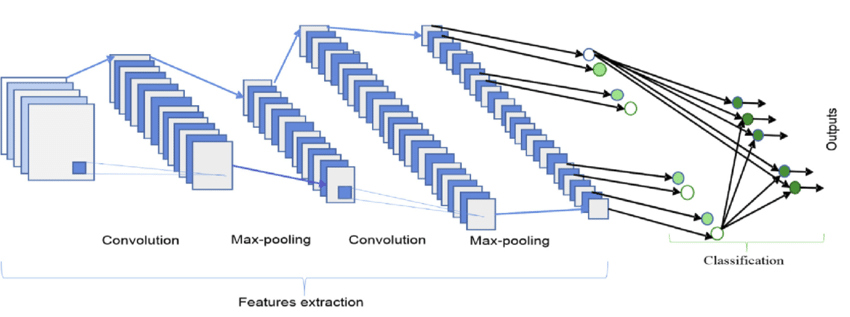
\includegraphics[scale=0.5]{cnn.png}
	\caption{Convolutional Neural Network consisting of two Convolution layers, two Max-Pooling layers, Flatten layer and two Fully-Connected (Dense) layers}
	\label{fig:cnn1}
\end{figure}

Most commonly used layers in CNN architectures are convolution layer, max-pooling layer, flatten layer, dense layer and dropout layer.

\subsection{Convolution Layer}

Convolution layer is the building block of the CNN architecture. Its primary purpose is to extract features from input image, such as edges, lines, curves, colors. As we go deeper inside the network, it starts identifying more complex features, such as shapes, objects. This layer consists of multiple filters (usually 3x3 matrices) whose parameters need to be learned, and it performs dot products between parts of an image and these filters.

\subsection{Max-Pooling Layer}

Max-Pooling layer is located after a series of convolution layers in CNN architecture. It is a downsampling method which reduces dimensionality, thus decreasing number of parameters and computational power needed in order to train the network, while retaining important features and patterns. It is achieved by applying a max filter to non-overlapping subregions (usually 2x2 matrices), thus reducing the size of each feature map by a factor of 2, and discarding 75\% of acivations in the process.

\subsection{Flatten Layer}

Output of the convolutional base of the network (series of convolution and max-pooling layers) is a two-dimensional matrix, and before feeding that data to the classification top of the network, it needs to be transformed. Flatten layer reshapes the output matrix to vector, thus removing all dimensions but one in the process, making the data prepared for the series of fully-connected layers.

\subsection{Fully-Connected Layer}

After the high-level features of the image have been detected, series of fully-connected (dense) layers is attached to the top of the network in order to classify image into a label. Dense layers consist of huge number of nodes (neurons), which provide a way of learning non-linear combinations of features outputted by convolutional base, and determine which feature most correlate to a particular class.

\subsection{Dropout Layer}

Fully-Connected layer contains the most parameters in the network, and as a result neurons develop co-dependency amongst each other during training, which leads to over-fitting the data (not generalizing well on new, unseen images). In order to prevent that, dropout layers are positioned right after dense layers in CNN architecture as a means of regularizing the network. Dropout consists of randomly ignoring (dropping out) fraction of neurons of fully-connected layer, which in turn makes network learn more robust features, and achieve better performance.
\clearpage

\subsection{CNNSimple Implementation}

CNNSimple convolutional neural network (\textcolor{red}{Code \ref{src:py1}}) was created using Keras Sequential model in order to classify images from NCT-CRC-HE-100K dataset, which contains 80.000 images divided into 9 tissue/cancer categories. 

Convolutional base of CNNSimple is composed of four blocks of convolution and max-pooling layers, where first two blocks have two convolution and one max-pooling layer, and last two blocks have three convolution and one max-pooling layer. Each convolution layer has 3x3 convolution window, uses ReLU activation function, and number of feature maps (filters) increases exponentially from 32 to 256. Each max-pooling layer has 2x2 pool size. 

Classification top of CNNSimple is composed of two fully-connected layers, each followed by a dropout layer, and an output (also fully-connected) layer. Fully-connected layers use ReLU activation function, and number of neurons grows from 512 to 1024. Dropout layers use 50\% dropout rate (fraction of neurons which will be ignored in each passing). Output layer uses softmax activation function, and has nine neurons (one neuron per tissue/cancer subtype output). 
\vspace{3mm}
\lstset{caption={CNNSimple network architecture},label=src:py1}
\begin{lstlisting}[language={Python}, basicstyle=\scriptsize]
	model = Sequential()
	model.add(Conv2D(32, (3, 3), activation='relu', input_shape=input_shape,     
	                 name='block1_conv1'))
	model.add(Conv2D(32, (3, 3), activation='relu', name='block1_conv2'))
	model.add(MaxPooling2D((2, 2), name='block1_pool'))
	model.add(Conv2D(64, (3, 3), activation='relu', name='block2_conv1'))
	model.add(Conv2D(64, (3, 3), activation='relu', name='block2_conv2'))
	model.add(MaxPooling2D((2, 2), name='block2_pool'))
	model.add(Conv2D(128, (3, 3), activation='relu', name='block3_conv1'))
	model.add(Conv2D(128, (3, 3), activation='relu', name='block3_conv2'))
	model.add(Conv2D(128, (3, 3), activation='relu', name='block3_conv3'))
	model.add(MaxPooling2D((2, 2), name='block3_pool'))
	model.add(Conv2D(256, (3, 3), activation='relu', name='block4_conv1'))
	model.add(Conv2D(256, (3, 3), activation='relu', name='block4_conv2'))
	model.add(Conv2D(256, (3, 3), activation='relu', name='block4_conv3'))
	model.add(MaxPooling2D((2, 2), name='block4_pool'))
	model.add(Flatten(name='flatten'))
	model.add(Dense(512, activation='relu', name='dense1'))
	model.add(Dropout(0.5, name='dropout1'))
	model.add(Dense(1024, activation='relu', name='dense2'))
	model.add(Dropout(0.5, name='dropout2'))
	model.add(Dense(9, activation='softmax', name='prediction'))
\end{lstlisting} 

\subsection{Transfer Learning}

Although CNNs are a powerful tool for image classification, in order to achieve high accuracy, large amount of data is needed. Problem occurs when only small dataset is available (as is often in healthcare, ex. BreakHis dataset). In such cases transfer learning can be used: take model trained on large dataset and transfer knowledge to small dataset, i.e. freeze convolutional base, and only train classification top of the network. Main idea is that early layers of convolutional base learns low-level features applicable across all images, such as edges and patterns.

\subsection{VGG19Simple Implementation}

VGG19Simple convolutional neural network (\textcolor{red}{Code \ref{src:py2}}) was created using Keras Graphical API in order to classify images from BreakHis dataset, which contains 2.000 images divided into 8 tissue/cancer categories. 

Convolutional base of VGG19Simple is VGG19 pre-built network pre-trained on ImageNet dataset (without top classification part), using imagenet weights.

Classification top of CNNSimple is composed of two fully-connected layers, each followed by a dropout layer, and an output (also fully-connected) layer. Fully-connected layers use ReLU activation function, and number of neurons grows from 512 to 1024. Dropout layers use 50\% dropout rate (fraction of neurons which will be ignored in each passing). Output layer uses softmax activation function, and has nine neurons (one neuron per tissue/cancer subtype output). 

\vspace{3mm}
\lstset{caption={VGG19Simple network architecture},label=src:py2}
\begin{lstlisting}[language={Python}, basicstyle=\scriptsize]
	input = Input((150, 150, 3))
	convolutional_base = VGG19(weights='imagenet', include_top=False,
	                           input_tensor=input)
	for layer in convolutional_base.layers:
		layer.trainable = False
	x = Flatten(name='flatten')(convolutional_base.output)
	x = Dense(512, activation='relu', name='dense_1')(x)
	x = Dropout(0.5, name='dropout_1')(x)
	x = Dense(1024, activation='relu', name='dense_2')(x)
	x = Dropout(0.5, name='dropout_2')(x)
	x = Dense(8, activation='softmax', name='predictions')(x)
	
	model = Model(input, x)
\end{lstlisting} 

\section{Experiments and Results}

Performance of neural networks is determined by how well will it generalize, i.e. how high accuracy will it achieve on previously unseen data (if it performs well on training data, but underachieves on test data, it is said that CNN overfits). In order to prevent overfitting, number of techniques can be used: increase size of dataset, change network architecture or apply hyperparameter tuning techniques, which consist of selecting a set optimal hyperparameters for learning algorithm. Selection of such parameters for networks is done in \textbf{\emph{hyperparameter\_tuning.py}}. First step consists of defining hyperparameter dictionary with parameters and values to be tested, such as number of epochs for which network is to be trained, optimization techniques, etc. Next step consists of training network with all combination of parameters and values defined, after which network performances are compared in order to determine the best hyperparameter set.

CNNSimple network trained on NCT-CRC-HE-100K dataset was trained for 50 epochs, using RMSProp optimizer with learning rate of 0.00002, using categorical crossentropy loss function. Before feeding data to the network, data augmentation (applying random transformations in order to produce more images, such as translation, rotation, sheer) has been used. In order to judge performance of the network, accuracy metrics function was employed. CNNSimple achieved 91.3\% validation and 91.3\% test accuracy, and 0.18 validation and 0.28 test loss (\textcolor{red}{\autoref{fig:cnnperf}}).

\begin{figure}[h]
	\centering
	\subfigure[\scriptsize Accuracy]{\label{fig:a}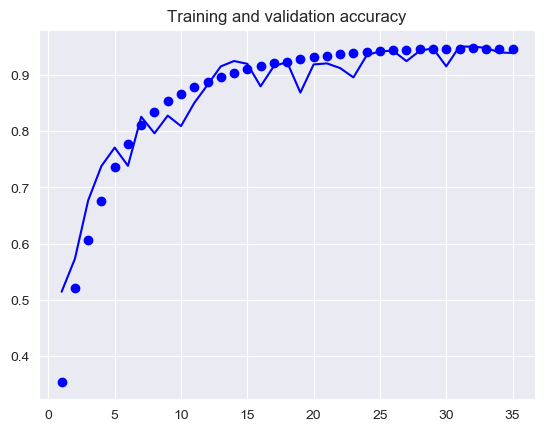
\includegraphics[width=65mm]{cnn_acc.png}}
	\subfigure[\scriptsize Loss]{\label{fig:b}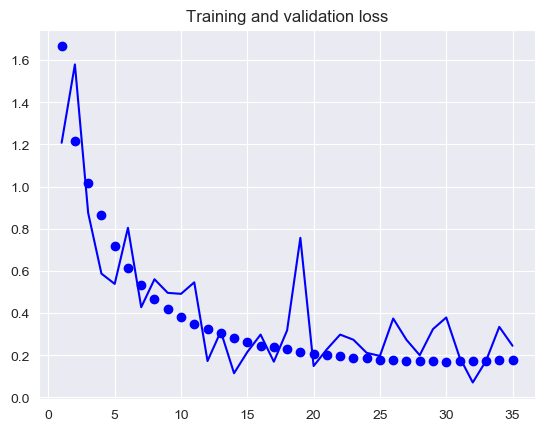
\includegraphics[width=65mm]{cnn_loss.png}}
	\caption{CNNSimple performance on NCT-CRC-HE-100K train and validation dataset}
	\label{fig:cnnperf}
\end{figure}

\clearpage
VGG19Simple network trained on BreakHis dataset was trained for 150 epochs, using Adam optimizer with learning rate of 0.0001, using categorical crossentropy loss function. Before feeding data to the network, data augmentation (applying random transformations in order to produce more images, such as translation, rotation, sheer) has been used. In order to judge performance of the network, accuracy metrics function was employed. After training network with frozen convolutional base, last convolutional block was unfreezed, and network was trained again using Adam optimizer with learning rate of 0.00005. VGG19Simple achieved 61.7\% validation and 62.1\% test accuracy, and 1.18 validation and 0.62 test loss (\textcolor{red}{\autoref{fig:vgg19perf}}).

\begin{figure}[h]
	\centering
	\subfigure[\scriptsize Accuracy]{\label{fig:vgg19perf}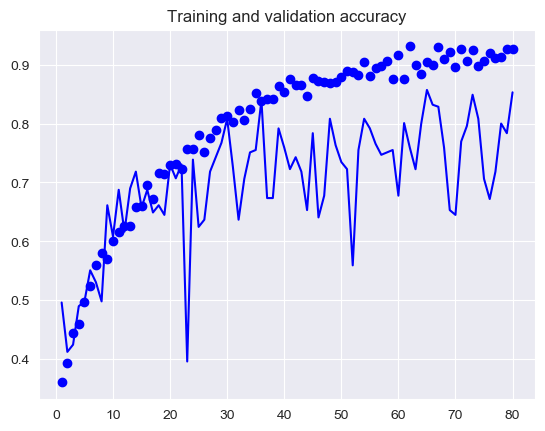
\includegraphics[width=65mm]{vgg19_acc.png}}
	\subfigure[\scriptsize Loss]{\label{fig:b}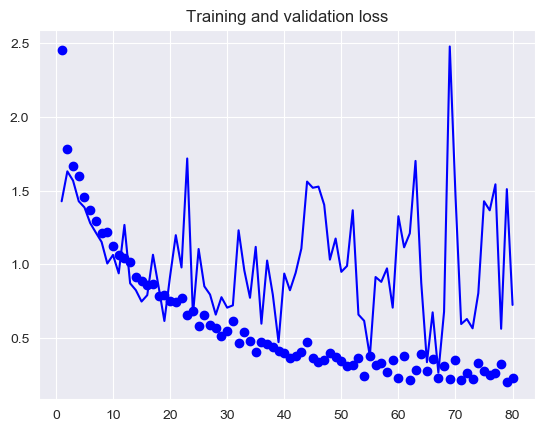
\includegraphics[width=65mm]{vgg19_loss.png}}
	\caption{VGG19Simple performance on BreakHis train and validation dataset}
	\label{fig:vgg19perf}
\end{figure}

Another way of interpreting network performance is by plotting confusion matrix, which is a summary table of correct and incorrect predictions broken down by each class (\textcolor{red}{\autoref{fig:cnncf}, \autoref{fig:vgg19cf}}).

\begin{figure}[h]
	\centering
	\begin{minipage}{.5\textwidth}
		\centering
		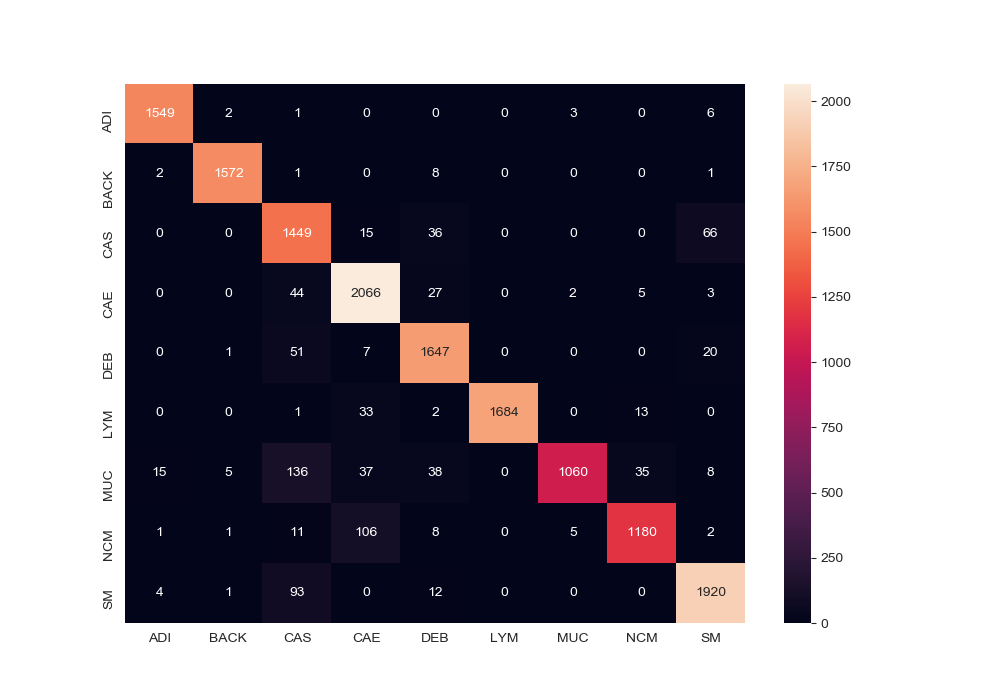
\includegraphics[scale=0.31]{cnn_cf.png}
		\captionof{figure}{Confusion Matrix of CNNSimple on NCT-CRC-HE-1OOK test dataset}
		\label{fig:cnncf}
	\end{minipage}%
	\begin{minipage}{.5\textwidth}
		\centering
		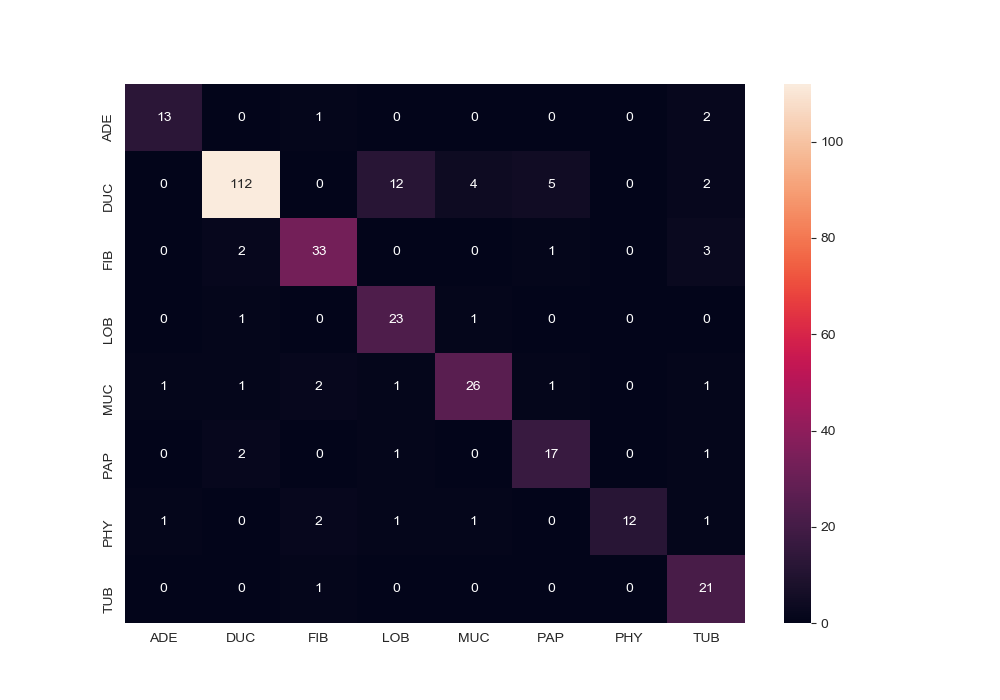
\includegraphics[scale=0.31]{vgg19_cf.png}
		\captionof{figure}{Confusion Matrix of VGG19Simple on BreakHis test dataset}
		\label{fig:vgg19cf}
	\end{minipage}
\end{figure}

\clearpage

\section{Graphical User Interface} \label{gui}

Text.

\section{Implementing Additional Features}

In addition to the ease of use of Histopathologic Cancer Detection program, source code was written in such a way to make expanding scope (problem space) of the program by including additional features quite simple and fast. If new tissue type, along with tissue/cancer subtype classification was to be added to the program, it would be done in four steps:
\begin{enumerate}
	\itemsep 0em
	\item Creating dataset \\
	...
	\item Building neural network \\
	...
	\item Choosing optimal hyperparameters \\
	...
	\item Extending graphical user interface \\
	...
\end{enumerate}

